\chapter{Справочное описание базовых нейросетевых архитектур обработки осциллограмм}
\label{app:base_ml_architectures}

В настоящем приложении приведено подробное описание структуры,
математических операций и параметров трёх базовых нейросетевых архитектур
глубокого обучения (\text{SimpleMLP}, \text{SimpleCNN} и \text{ResNet1D}),
используемых в главе~\ref{ch:oscillogram_analysis} в качестве эталона при
оценке разработанных физически-информированных моделей. Изложение
адаптировано применительно к задачам цифровой обработки многоканальных
записей токов и напряжений в устройствах РЗА и БАВР.

\section{Полносвязная нейронная сеть SimpleMLP}
\label{sec:app_simplemlp}

Полносвязный многослойный персептрон (\text{SimpleMLP}) представляет
собой базовую архитектуру, в которой все отсчёты всех измерительных
каналов анализируемого окна обрабатываются совместно в виде единого
вектора признаков. Последовательность преобразований в модели
\text{SimpleMLP} представлена на рисунке~\ref{fig:ch4_mlp_flow}.

\begin{figure}[htbp]
    \centering
    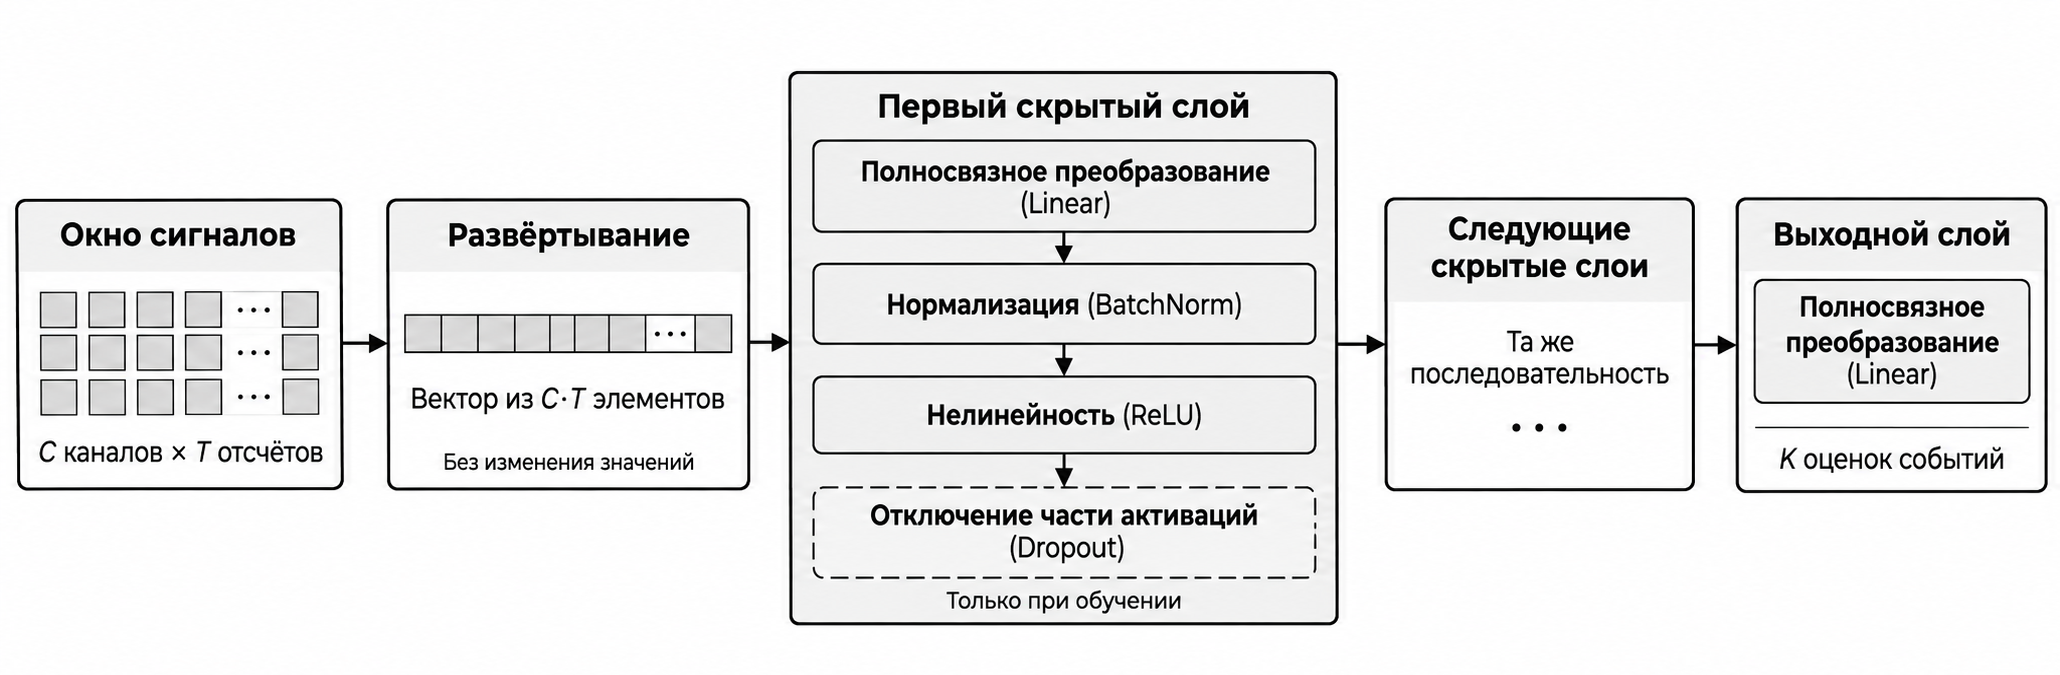
\includegraphics[width=\textwidth]{figures/appendix_a/physkan_mlp.png}
    \caption{Последовательность обработки окна осциллограммы в базовой
    полносвязной модели SimpleMLP}
    \label{fig:ch4_mlp_flow}
\end{figure}

На первом шаге выполняется операция развёртывания (Flatten), которая не
вычисляет новых физических величин, а последовательно размещает строки
входной матрицы $X\in\mathbb{R}^{C\times T}$ в один вектор-столбец
$\boldsymbol{x}$ размерности $n = C \cdot T$. Каждая компонента $x_i$
этого вектора жёстко соответствует определённому измерительному каналу
(например, току фазы $A$) и конкретному моменту времени внутри окна.

Далее вектор проходит через каскад полносвязных (линейных) слоёв. В
каждом слое формируется взвешенная сумма всех входных компонент со
свободным смещением $b_j$, после чего применяется нелинейная функция
активации $\operatorname{ReLU}(z)=\max(0,z)$, отсекающая отрицательные
значения отклика. Для стабилизации масштаба внутренних сигналов между
линейным преобразованием и функцией активации включается блок пакетной
нормализации (BatchNorm, BN), который центрирует и нормирует распределение
признаков по обучающим примерам. На этапе обучения после активации
дополнительно применяется процедура случайного прореживания (Dropout),
временно обнуляющая заданную долю нейронов слоя. В отличие от физического
отключения каналов при проверке отказов измерительных трансформаторов,
Dropout используется исключительно во время настройки весов для
предотвращения переобучения сети на частных особенностях отдельных
осциллограмм. При работе обученной модели в режиме прямого расчёта
случайное отключение полностью выводится из работы.

Общее число обучаемых параметров (весов и смещений) одного полносвязного
слоя с $n$ входами и $m$ выходами составляет $(n+1)m$. Например, уже при
обработке короткого окна длительностью в один период промышленной частоты
(6~каналов по 32~отсчёта, $n=192$) первый скрытый слой из $m=64$ нейронов
требует настройки $(192+1)\cdot 64 = 12\,352$ коэффициентов (без учёта
параметров нормализации). При увеличении длины окна наблюдения число
параметров первого слоя растёт прямо пропорционально числу отсчётов $T$,
что повышает вычислительную ресурсоёмкость модели.

\section{Одномерная свёрточная нейронная сеть SimpleCNN}
\label{sec:app_simplecnn}

В отличие от полносвязной сети, свёрточная архитектура \text{SimpleCNN}
сохраняет разделение входных данных на ось измерительных каналов и ось
времени. Основная идея модели заключается в обработке сигнала короткими
скользящими фильтрами (ядрами свёртки), которые последовательно
перемещаются вдоль временной оси окна с фиксированным шагом. Структурная
схема обработки данных в \text{SimpleCNN} приведена на
рисунке~\ref{fig:ch4_cnn_flow}.

\begin{figure}[htbp]
    \centering
    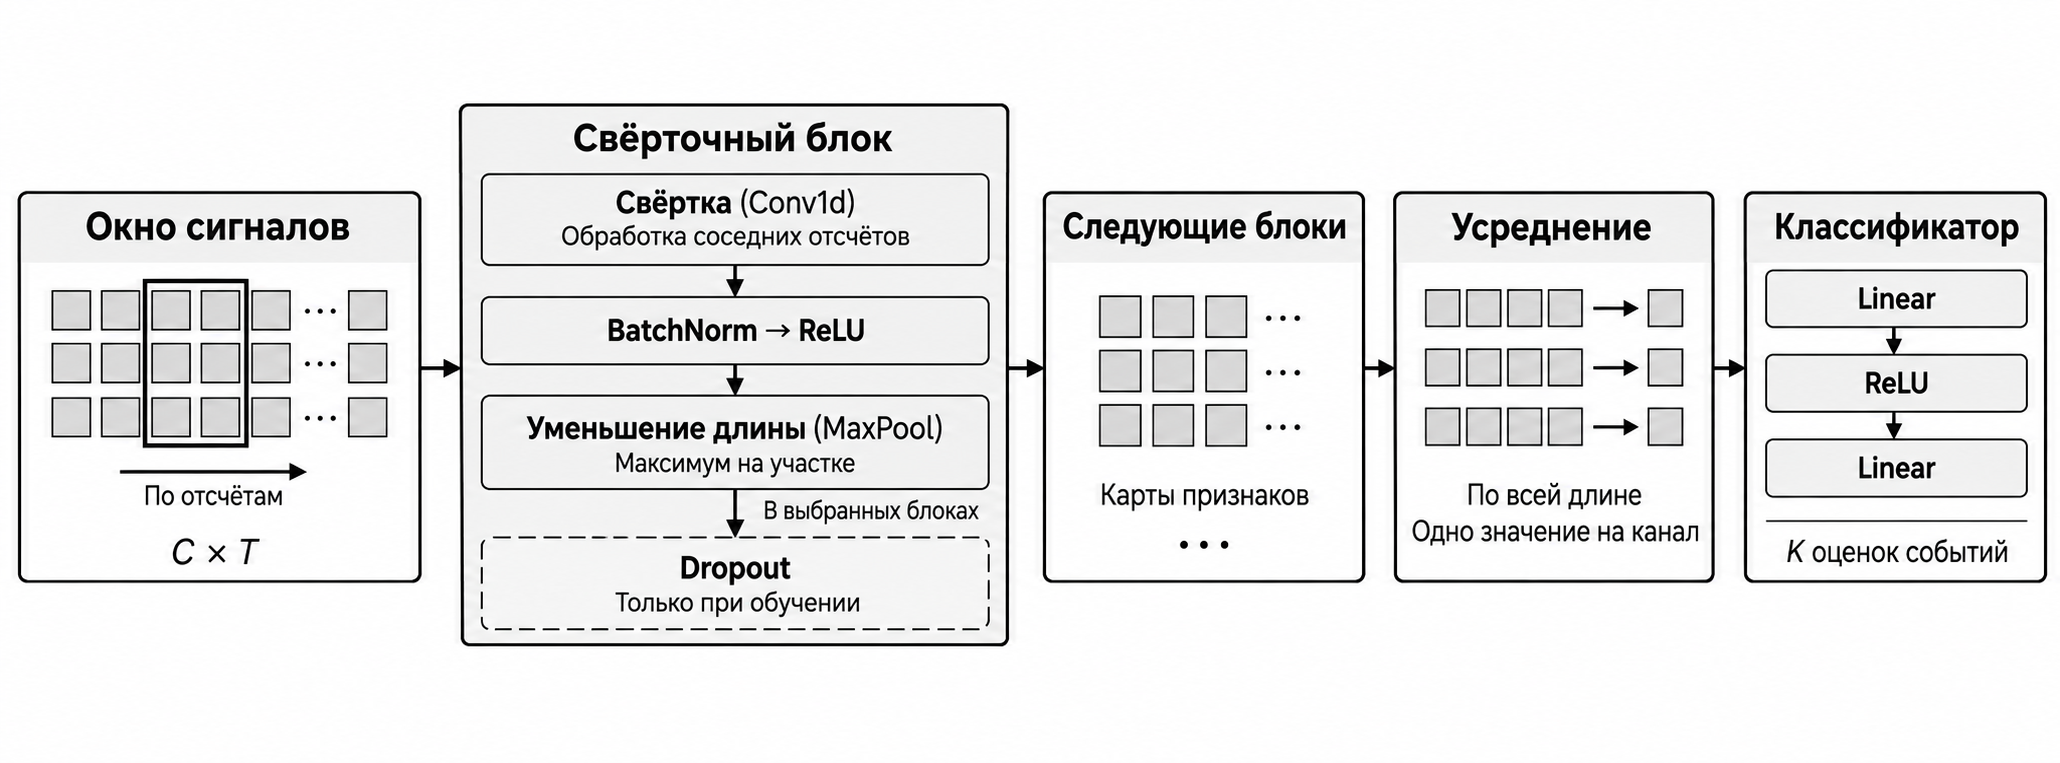
\includegraphics[width=\textwidth]{figures/appendix_a/physkan_cnn.png}
    \caption{Последовательность обработки окна в одномерной свёрточной
    модели SimpleCNN с выделением локальных признаков и усреднением вдоль
    временной оси}
    \label{fig:ch4_cnn_flow}
\end{figure}

Каждый выходной канал свёрточного слоя (называемый картой признаков)
формируется путём суммирования локальных участков всех входных каналов с
обучаемыми весовыми коэффициентами ядра длины $k$. Поскольку один и тот
же набор весов применяется ко всем временным участкам окна, число
параметров свёрточного слоя не зависит от длительности анализируемой
записи $T$. Так, при шести входных сигналах ($C=6$), шестнадцати
формируемых картах признаков и длине ядра $k=3$~отсчёта первый свёрточный
слой содержит всего $16\cdot(6\cdot 3 + 1) = 304$ обучаемых веса и
смещения, что на два порядка меньше, чем в аналогичном слое
\text{SimpleMLP}.

После каждого свёрточного преобразования, нормализации BatchNorm и
активации $\operatorname{ReLU}$ в выбранных каскадах выполняется операция
локального агрегирования по максимуму (MaxPool). Она выбирает наибольшее
значение отклика на коротком интервале соседних отсчётов, сжимая длину
временной последовательности и повышая устойчивость выделенных признаков
к малым фазовым сдвигам сигнала. По мере прохождения через несколько
свёрточных каскадов каждый отклик объединяет информацию со всё более
широкого интервала исходной осциллограммы, переходя от фиксации
мгновенных скачков тока и напряжения к распознаванию формы полуволны и
огибающей переходного процесса. На выходе свёрточной части выполняется
адаптивное усреднение каждой карты признаков по всей длине окна (Global
Average Pooling), после чего компактный вектор поступает в двухслойный
полносвязный классификатор.

\section{Одномерная остаточная нейронная сеть ResNet1D}
\label{sec:app_resnet}

При дальнейшем увеличении числа последовательно соединённых свёрточных
слоёв в обычной сети возникает проблема затухания градиентов при обучении
и деградации точности, когда глубокая модель начинает хуже передавать
исходную информацию о форме сигнала. Для устранения этого ограничения в
архитектуре \text{ResNet1D} используются остаточные блоки с обходными
(шунтирующими) связями, схема которых показана на
рисунке~\ref{fig:ch4_residual_flow}.

\begin{figure}[htbp]
    \centering
    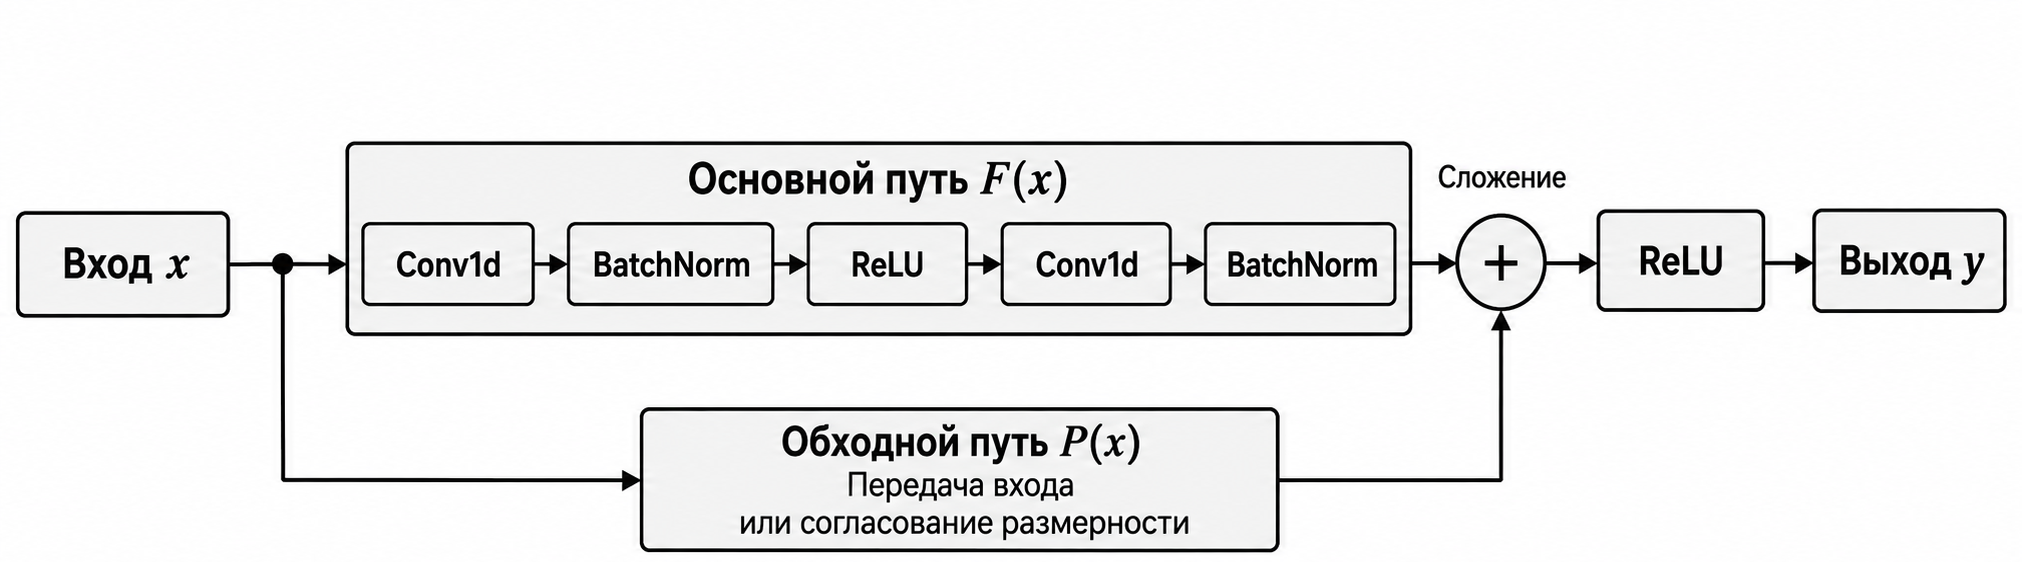
\includegraphics[width=\textwidth]{figures/appendix_a/physkan_residual.png}
    \caption{Структура остаточного блока модели ResNet1D с основным
    свёрточным путём и обходной связью}
    \label{fig:ch4_residual_flow}
\end{figure}

В каждом остаточном блоке сигнал разветвляется на два параллельных
канала. В основном канале последовательно выполняются две одномерные
свёртки с пакетной нормализацией и промежуточной активацией
$\operatorname{ReLU}$, формирующие нелинейную поправку $F(\boldsymbol{x})$
к текущему представлению сигнала. По обходному каналу передаётся сам
входной вектор блока $\boldsymbol{x}$ (либо его линейная проекция
$P(\boldsymbol{x})$ с помощью точечной свёртки с ядром единичной длины в
тех случаях, когда в блоке изменяется число каналов или шаг по времени).
На выходе блока оба канала суммируются, что позволяет без искажений
транслировать как сами признаки в прямом направлении, так и производные
ошибки в обратном направлении при обучении.

Полная архитектура рассматриваемой модели \text{ResNet1D} включает
входной свёрточный каскад предварительного сжатия и четыре
последовательные остаточные ступени, в которых количество карт признаков
поэтапно увеличивается относительно базового числа каналов в пропорции
$1:2:4:8$. После четвёртой ступени, аналогично \text{SimpleCNN},
выполняется глобальное усреднение по времени и линейная классификация
событий.